\section{Deep Learning-Based Segmentation Algorithms} \label{ssec:segmentation}
In digital image processing, image segmentation is the process of recognizing and subdividing an image into different regions of pixels that show similar features, like color, texture, or intensity. Typically, the task of segmentation is to recognize the edges and boundaries of the different objects in the image and assigning a different label to every detected region. The result of the segmentation process is an image with the same dimensions of the starting one made of solid color regions, representing the detected objects. This image is called \textit{segmentation mask}. In Figure \ref{fig:seg_example} is shown an example of segmentation of a picture of an urban landscape: different colors are linked to different classes of objects like persons in magenta and scooters in purple. This technology has a significant role in a wide variety of application fields such as scene understanding, medical image analysis, augmented reality, etc.

\begin{figure}
    \centering
    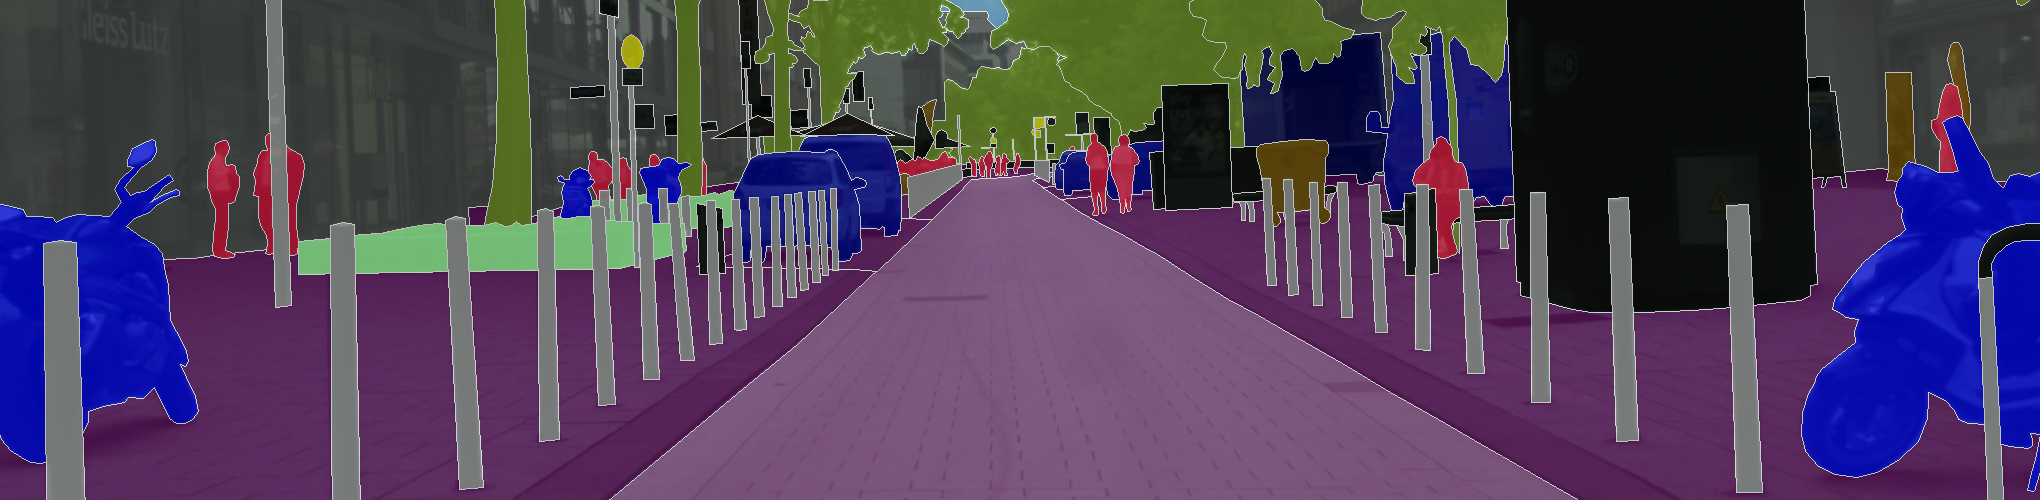
\includegraphics[width = \textwidth]{images/seg_example}
    \caption{Example of the resulting segmentation mask of an image of an urban landscape. Every interesting object of the image is detected and a solid color region replaces it in the segmentation mask. Every color corresponds to a different class of objects, for example, persons are highlighted in magenta and scooters in purple. The shape and the boundaries of every region should match as precisely as possible the edges of the objects.}
    \label{fig:seg_example}
\end{figure}

A relatively easy problem, and one of the first to be tackled, could be distinguishing an object from the background in a grey-scale image. The easiest technique to perform segmentation in this kind of problem is based on thresholding. Thresholding is a binarization technique based on the image's grey-level histogram: to every pixel with luminosity above that threshold is assigned the color \textit{white}, and vice versa the color \textit{black}. However, this is a very primitive and fallacious, yet very fast method, and it manages poorly complex images or images with un-uniformity in the background.

A lot of other traditional techniques improve this first segmentation method \cite{Chouhan2018}. Some are based on the object's edges recognition, exploiting the sharp change in luminosity typically in correspondence of the boundary of a shape. Other techniques exploit instead a region-growing technology, according to which some \textit{seed} region markers are scattered on the image, and the regions corresponding to the objects in the image are grown to incorporate adjacent pixels with similar properties.

\begin{figure}
    \centering
    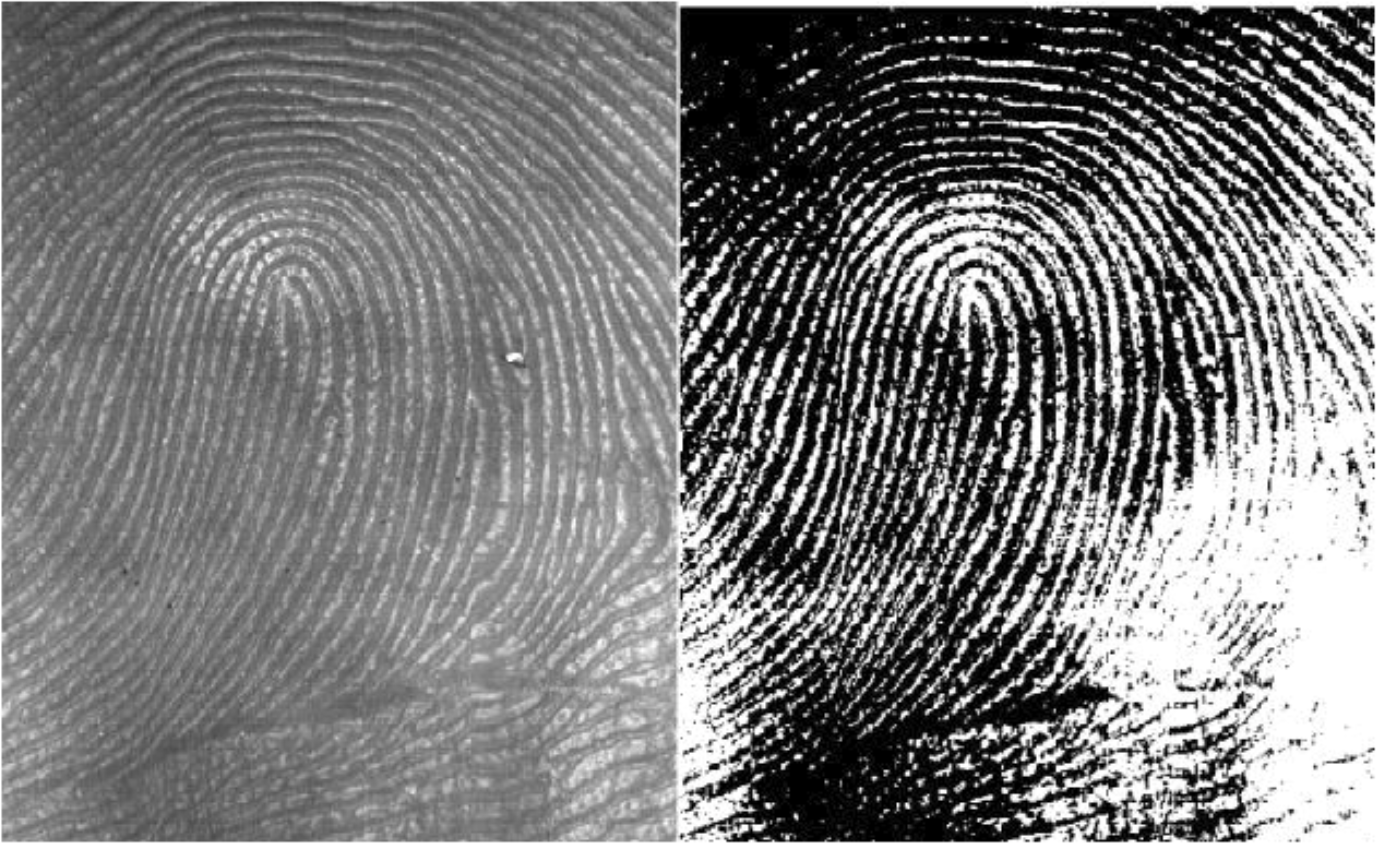
\includegraphics[width = 0.7\textwidth]{images/fingerprints}
    \caption{Example of the resulting segmentation mask of an image of a fingeprint obtained trhough a thresholding algorithm. The result is not extremely good, but this techinque is very easy to implement and runs very quickly.}
    \label{fig:fing_prints}
\end{figure}

\subsection{State of the Art on Deep Learning Segmentation} \label{ssec:soa_seg}
Similarly to many other traditional tasks, also for segmentation, there has been a thriving development lead by the diffusion of deep learning, that boosted the performances resulting in what many regards as
a paradigm shift in the field \cite{deep_seg_SOA}.

In further detail, image segmentation can be formulated as a classification problem of pixels with semantic labels (semantic segmentation) or partitioning of individual objects (instance segmentation). Semantic segmentation performs pixel-level labeling with a set of object categories (e.g. boat, car, person, tree) for all the pixels in the image, hence it is typically a harder task than image classification, which requires just a single label for the whole image. Instance segmentation extends semantic segmentation scope further by detecting and delineating each object of interest in the image (e.g. partitioning of individual nuclei in a histological image).

There are many prominent Neural Network architectures used in the computer vision community nowadays, based on very different ideas such as convolution, recursion, dimensionality reduction, and image generation. This section will provide an overview of the state of the art of this technology and will dwell briefly on the details behind some of those innovative architectures.

\begin{description}
    \item [Recurrent Neural Networks (RNNs) and the LSTM] \hfill \\
        The typical application for RNN is processing sequential data, as written text, speech or video clips, or any other kind of time-series signal. In this kind of data, there is a strong dependency between values at a given time/position and values previously processed. Those models try to implement the concept of \textit{memory} weaving connections, outside the main information flow of the network, with the previous NN's input. At each time-stamp, the model collects the input from the current time $X_i$ and the hidden state from the previous step $h_{i-1}$ and outputs a target value and a new hidden state (Figure \ref{fig:recNN}). Typically RNN cannot manage easily long-term dependencies in long sequences of signals. There is no theoretical limitation in this direction, but often it arises vanishing (or exploding) gradient problematics during the training phase. A specific type of RNN has been designed to avoid this situation, the so-called Long Short Term Memory (LSTM) \cite{LSTM}. The LSTM architecture includes three gates (input gate, output gate, forget gate), which regulate the flow of information into and out from a memory cell, which stores values over arbitrary time intervals.

        \begin{figure}
            \centering
            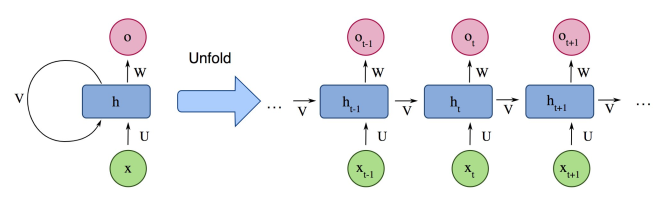
\includegraphics[width = 0.8\textwidth]{images/recNN}
            \caption{Example of the structure of a simple Recurrent Neural Network from  \cite{deep_seg_SOA}.}
            \label{fig:recNN}
        \end{figure}

    \item [Encoder-Decoder and Auto-Encoder Models] \hfill \\
        Encoder-Decoder models try to learn the relation between an input and the corresponding output with a two steps process. The first step is the so-called \textit{encoding} process, in which the input $x$ is compressed in what is called the \textit{latent-space} representation $z = f(x)$. The second step is the \textit{decoding} process, where the NN predicts the output starting from the latent-space representation $ y = g(z)$. The idea underneath this approach is to capture in the latent-space representation the underlying semantic information of the input that is useful for predicting the output. ED models are widely used in image-to-image problems (where both input and output are images) and for sequential-data processing (like Natural Language Processing, NLP). In Figure \ref{fig:EDNN} is shown a schematic representation of this architecture. Usually, these model follow a supervised training, trying to reduce the reconstruction loss between the predicted output and the ground-truth output provided while training. Typical applications for this technology are image-enhancing techniques like de-noising or super-resolution, where the output image is an improved version of the input image. Or image generation problems (e.g. plausible new human faces generation) in which all the properties which define the type of image under analysis should be learned in the representation latent space.

        \begin{figure}
            \centering
            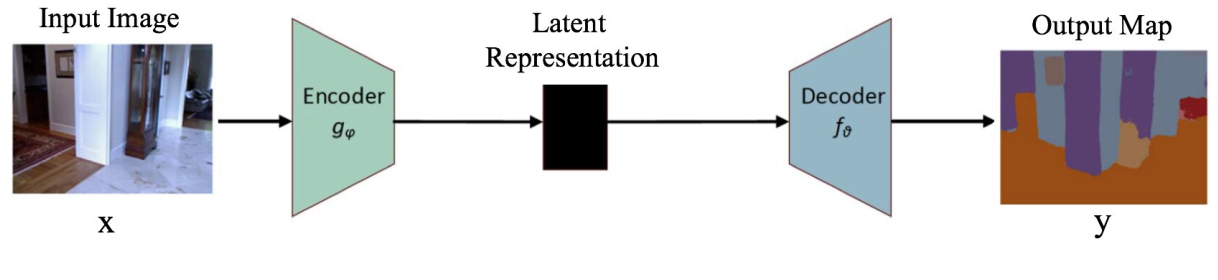
\includegraphics[width = 0.8\textwidth]{images/EDnet}
            \caption{Example of the structure of a simple Encoder-Decoder Neural Network from  \cite{deep_seg_SOA}.}
            \label{fig:EDNN}
        \end{figure}

    \item [Generative Adversarial Networks (GANs)] \hfill \\
        The peculiarity of Generative Adversarial Network (GAN) lies in its structure. It is actually made of two distinct and independent modules: a generator and a discriminator, as shown in Figure \ref{fig:GAN}. The first module $G$, responsible for the generation, typically learns to map a prior random distribution of input $z$ to a target distribution $y$, as similar as possible to the target $G = z \rightarrow y$ (i.e. almost any kind of image-to-image problem could be addressed with GANs, as in \cite{1611.07004}). The second module, the discriminator $D$, instead is trained to distinguish between \textit{real} and \textit{fake} images of the target category. These two networks are trained alternately in the same training process. The generator tries to fool the discriminator and vice versa. The name adversarial is actually due to this \textit{competition} within different parts of the network. The formal manner to set up this adversarial training lies in the accurate choice of a suitable loss function, that will look like: $$L_{GAN} = \mathbb{E}_{x \sim p_{data}(x)}[logD(x)] + \mathbb{E}_{z \sim p_{z}(z)}[log(1-D(G(z)))]$$.
        The GAN is thus based on a min-max game between $G$ and $D$. $D$ aims to reduce the classification error in distinguishing fake samples from real ones, and as a consequence maximizing the $L_{GAN}$. On the other hand, $G$ wants to maximize the $D$'s error, hence minimizing $L_{GAN}$. The result of the training process is the trained generator $G^*$, capable of produce an arbitrary number of new data (images, text, or whatever else): $$ G^* = \operatorname*{arg\,min_Gmax_D} L_{GAN}$$.
        This peculiar architecture has yielded several interesting results and it has been developed in many different directions, with influences and contaminations with other architectures \cite{1611.07004}.

        \begin{figure}
            \centering
            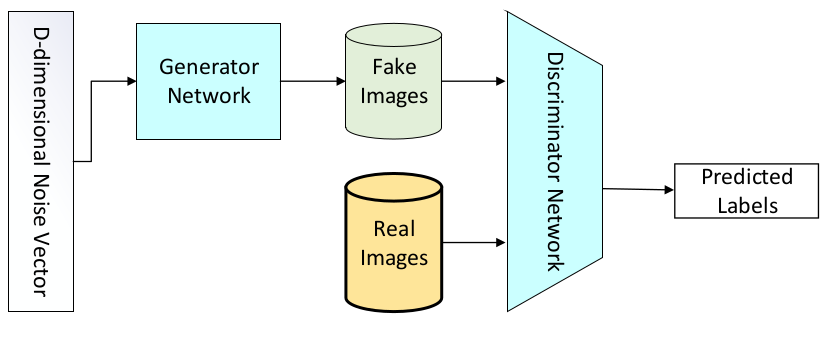
\includegraphics[width = 0.6\textwidth]{images/GAN}
            \caption{Schematical representation of a Generative Adversarial Networks, form \cite{deep_seg_SOA}.}
            \label{fig:GAN}
        \end{figure}

    \item [Convolutional Neural Networks (CNNs)] \hfill \\
        As stated before CNNs are a staple choice in image processing DL applications. They mainly consist of three types of layers:

        \begin{enumerate}[i]
            \item convolutional layers, where a kernel window of parameters is convolved with the image pixels and produce numerical features maps.

            \item nonlinear layers, which apply an activation function on feature maps (usually element-wise). This step allows the network to introduce non-linear behavior and then increasing its modeling capabilities.

            \item pooling layers, which replace a small neighborhood of a feature map with some statistical information (mean, max, etc.) about the neighborhood and reduce the spatial resolution.
        \end{enumerate}

        Given the arrangement of successive layers, each unit receives weighted inputs from a small neighborhood, known as the receptive field, of units in the previous layer. The stack of layers allows the NN to perceive different resolutions: the higher-level layers learn features from increasingly wider receptive fields. The leading computational advantage given by CNN architecture lies in the sharing of kernels' weights within a convolutional layer. The result is a significantly smaller number of parameters than fully-connected neural networks. In section \ref{ssec:sttrNN} will be shown a particular application of this architecture, known as \textit{style-transfer} network, which is a particular algorithm capable of implanting the visual texture of a \textit{style} image onto the content of a different image, producing interesting hybrid images. Some of the most notorious CNN architectures include: AlexNet \cite{AlexNet}, VGGNet \cite{1409.1556}, and U-Net \cite{U-net}.
\end{description}

For this work, U-net architecture is particularly interesting. The U-net model was initially developed for biomedical image segmentation, and in its structure reflects characteristics of both CNN and Encoder-Decoder models. Ronneberger et al.\cite{U-net} proposed this model for segmenting biological microscopy images in 2015. The U-Net architecture is made of two branches, a contracting path to capture context, and a symmetric expanding path (see Figure \ref{fig:unet}). The down-sampling flow is made of a Fully Convolutional Network (FCN)-like architecture that computes features with 3 $\times$ 3 kernel convolutions. On the other hand, the up-sampling branch exploits up-convolution operations (or deconvolution), reducing the number of feature maps while increasing their dimensions. Another characteristic of this architecture is the presence of direct connections between layers of a similar level of compression in compressing and decompressing branches. Those links allow the NN to preserve spatial and pattern information. The Network flow eventually ends with a 1 $\times$ 1 convolution layer responsible for the generation of the segmentation mask of the input image.

    \begin{figure}
        \centering
        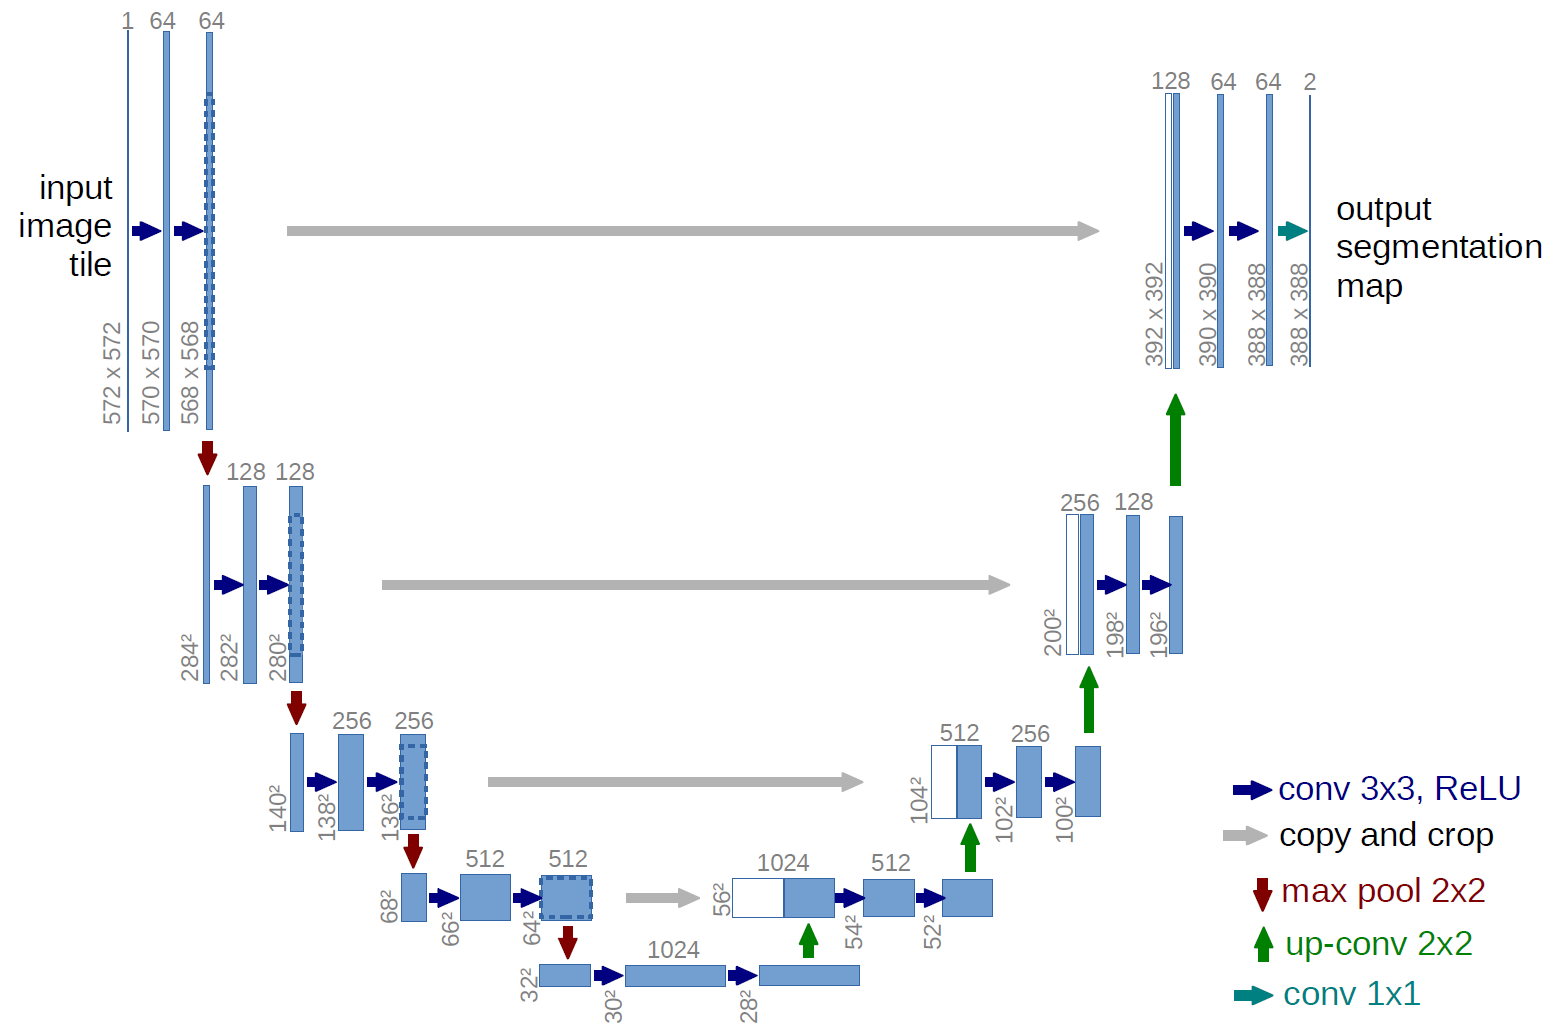
\includegraphics[width = 0.8\textwidth]{images/unet}
        \caption{Scheme of the typical architecture of a U-net NN. This particular model was firstly proposed by Ronneberger \textit{et al.} in \cite{U-net}.}
        \label{fig:unet}
    \end{figure}

\hl{I SHOULD REPORT HERE SOME ACTUAL RESULT OF SEGMENTATION OF HISTOLOGICAL SEGMENTATION TO CONCLUDE THE DISCUSSION. NUCLEI DETECTION OR SIMILA.}

    \begin{figure}
        \centering
        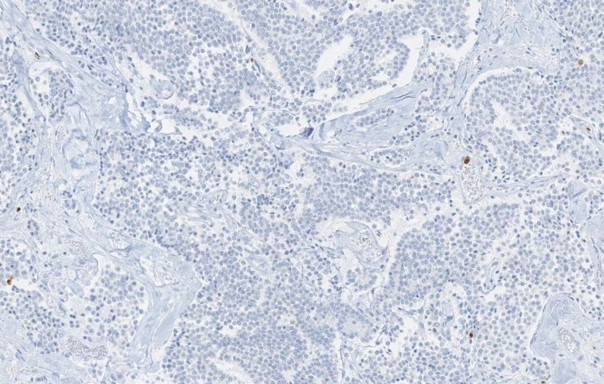
\includegraphics[width = 0.4\textwidth]{images/PancTissue}
        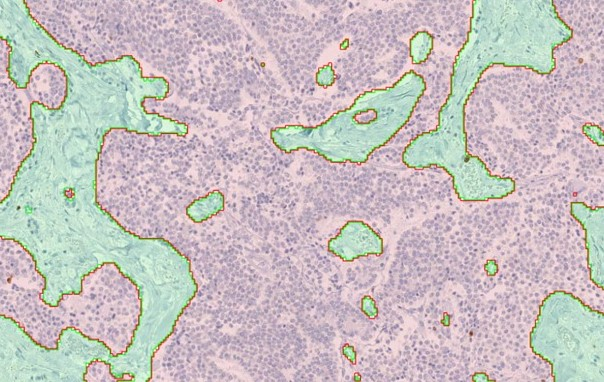
\includegraphics[width = 0.4\textwidth]{images/PancTissueSeg}
        \caption{}
        \label{fig:autom_seg}
    \end{figure}

\subsection{Image Segmentation Datasets}
Besides the choice of suitable architecture the most important aspect while developing a NN is the dataset on which perform the training process. Let confine the discussion only to image-to-image problems, like segmentation problems. There are a lot of widely used datasets, but I want to mention just a few of them to give the idea of their typical characteristics.

A good example of segmentation is the Cityscapes dataset \cite{Cityscapes}, which is a large-scale database with a focus on semantic understanding of urban street scenes. The dataset is made of video sequences from the point of view of a car in the road traffic, from 50 different cities in the world. The clips are made of 5K frames, labeled with extremely high quality at pixel-level and an additional set of 20K weakly-annotated frames. Each pixel in the segmentation mask contains the semantic classification, among over 30 classes of objects. An example of an image from this dataset is shown in Figure \ref{fig:seg_example}.

The PASCAL Visual Object Classes (VOC) \cite{PASCAL} is another of the most popular datasets in computer vision. This dataset is designed to support the training of algorithms for 5 different tasks: segmentation, classification, detection, person layout, and action recognition. In particular, for segmentation, there are over 20 classes of labeled objects (e.g. planes, bus, car, sofa, TV, dogs, person, etc.). The dataset comes divided into two portions: training and validation, with 1,464 and 1,449 images, respectively. In Figure \ref{fig:PASCAL} is shown an example of an image and its corresponding segmentation mask.

    \begin{figure}
        \centering
        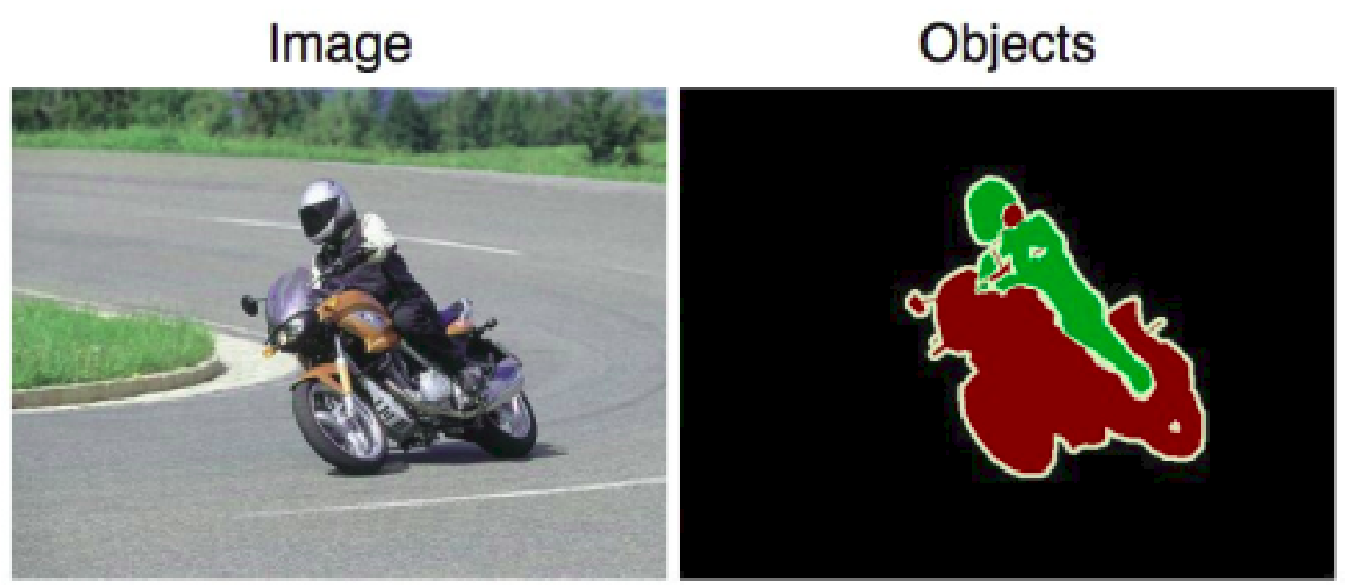
\includegraphics[width = 0.5\textwidth]{images/PASCAL}
        \caption{An example image from the PASCAL dataset and its corresponding segmentation mask \cite{PASCAL}.}
        \label{fig:PASCAL}
    \end{figure}

It is worth mentioning that in the medical image processing domain typically the available dataset is definitely not that rich and vast (that is actually the seed of this work) and thus many techniques of data augmentation have been devised, to get the best out of the restricted amount of material. Generally, data augmentation manipulates the starting material applying a set of transformation to create new material, like rotation, reflection, scaling, cropping and shifting, etc. Data augmentation has been proven to improve the efficacy of the training, making the model less prone to over-fitting, increasing the generalization power of the model, and helping the convergence to a stable solution during the training process.
